\chapter{Tijdreeksen}

In de voorgaande hoofdstukken hebben we telkens data geanalyseerd die op een bepaald moment in de tijd is verzameld en we hebben uitspraken gedaan over die data voor dat specifieke moment.

In de ict-beroepspraktijk zijn er echter ook vele toepassingen waar het nodig is om data op te volgen die voortdurend verandert. We denken dan bijvoorbeeld aan de belasting van een processor, evolutie van schijfgebruik op een opslagapparaat, de responstijd van een website, enz.

In dit hoofdstuk gaan we dit soort data onder de loep nemen en de belangrijkste analysemethoden bespreken.

\section{Tijdreeksen \& voorspellingen}

\begin{definition}[Tijdreeks]
Een \emph{tijdreeks} is een opeenvolging van observaties van een willekeurige variabele in functie van de tijd.
\end{definition}

Voorbeelden:

\begin{itemize}
	\item maandelijkse vraag naar melk
	\item jaarlijkse instroom van studenten bij de Hogeschool
	\item dagelijks debiet van een rivier
	\item de buitentemperatuur over het verloop van een dag
\end{itemize}

Het voorspellen van tijdreeksen is een belangrijk onderdeel van onderzoek omdat ze vaak de basis vormen voor beslissingsmodellen. Voorbeelden hiervan zijn:

\begin{itemize}
	\item algemene ontwikkeling van toekomstplannen (investeringen, capaciteit \dots)
	\item plannen van budgettering om tekortkomingen te vermijden (operationeel budget, marketing budget \dots)
	\item competitieve leveringstijden van een bedrijf
	\item ondersteuning van financiële objectieven
	\item onzekerheid vermijden
	\item de mogelijkheid om ontwikkelingen in de verkeersveiligheid
kwantitatief te modelleren
\end{itemize}

Tijdreeksen modelleren is een statistisch probleem: we gaan ervan uit dat de observaties variëren volgens een bepaalde kansdichtheidsfunctie in functie van de tijd. Vaak gaan we ervan uit dat de observaties in een tijdreeks gecorreleerd zijn en dus niet uit een willekeurige steekproef komen. 

Er zijn verschillende types modellen in gebruik voor het analyseren van tijdreeksen. Deze modellen hebben met elkaar gemeen dat ze in principe niet alleen de ontwikkeling in een geobserveerde tijdreeks kunnen beschrijven, maar dat we ze ook kunnen gebruiken om
\begin{inparaenum}[(i)]
	\item verklaringen te vinden voor die ontwikkeling en
	\item om de toekomstige waarden van de tijdreeks te voorspellen.
\end{inparaenum}
Hun geschiktheid voor het verwezenlijken van deze doelstellingen loopt echter sterk uiteen. In dit hoofdstuk beperken we ons tot het gebruik van tijdreeksen met een geschiedenis om tijdsafhankelijke modellen te bepalen. Een voorbeeld van een tijdreeks is bijvoorbeeld de leeftijd van de opeenvolgende koningen van Engeland startend van Willem De Veroveraar \autocite{Hipel1994}.

\begin{lstlisting}
kings <- scan(file = 'cursus/data/tijdreeksen/kings.data', skip = 3)
kingstimeseries <- ts(kings)
plot.ts(kingstimeseries, ylab='leeftijd', xlab="tijd")
grid(lty=2,lwd=1,col='black')
\end{lstlisting}

\begin{figure}
	\centering
	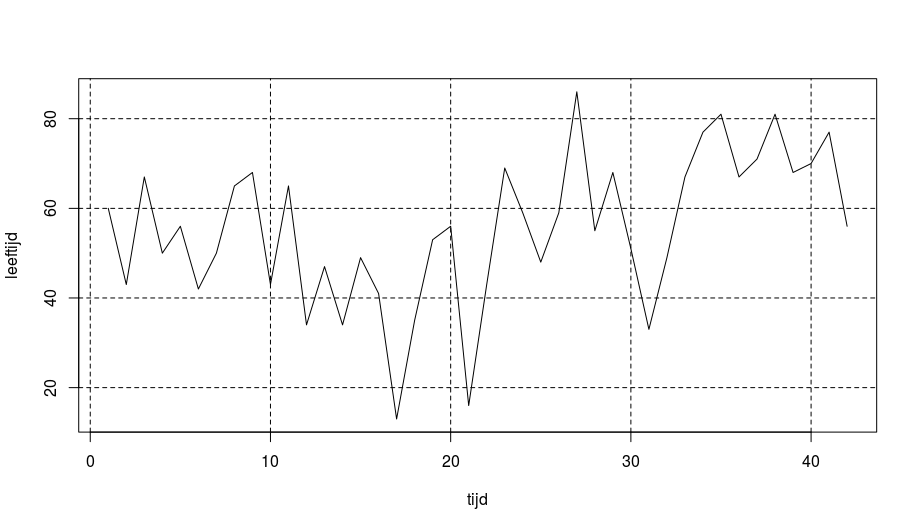
\includegraphics[width=\textwidth]{images/tijdreeksen/tijdreekskings.png}
	\caption{De tijdreeks die de leeftijden van de koningen voorstelt.}
	\label{fig:tijdreeks11}
\end{figure}

\section{Tijdreeksmodellen}

\subsection{Wiskundig model}

Ons doel is het opstellen van een model dat een verklaring vindt voor de geobserveerde data en dat toelaat om observaties in de toekomst zo goed mogelijk te voorspellen. Het simpelste model dat je kan bedenken is een model waarbij een constante $b$ gebruikt wordt met variaties rond $b$ bepaald door een willekeurige variabele $\epsilon_{t}$ zoals in vergelijking~\ref{eq:constante}. 

\begin{equation}
	X_{t} = b + \epsilon_{t}
\label{eq:constante}
\end{equation}

\begin{description}
  \item [$X_{t}$] stelt een \emph{variabele} voor dat de onbekende is op tijdstip $t$.
  \item [$x_{t}$] stelt een \emph{observatie} voor op tijdstip $t$ (en is dus gekend). 
  \item [$\epsilon_{t}$] noemt met de \emph{storing} (Eng. \emph{noise}) en wordt geacht een gemiddelde van $0$ te hebben met variantie $\sigma^{2}$ en normaal verdeeld ($\epsilon_{t} \sim Nor(0, \sigma)$). 
\end{description}

We kunnen ook ervan uit gaan dat er een lineair verband is:

\begin{equation}
X_{t} = b_{0} + b_{1} \times t + \epsilon_{t}
\label{eq:lineair8}
\end{equation}

De vergelijking in \ref{eq:constante} en \ref{eq:lineair8} zijn speciale gevallen van het polynomiaal geval:

\begin{equation}
	X_{t} = b_{0} + b_{1} t + b_{2} t^{2} + \dots + b_{n} t^{n} + \epsilon_{t} 
\label{eq:polynomiaal}
\end{equation}

\begin{exercise}
	Wat zou volgende tijdreeks kunnen voorstellen?
	\begin{equation}
		X_{t} = b_{0} + b_{1} \sin\left(\frac{2\pi t}{4}\right) + b_{1} \cos\left(\frac{2\pi t}{4}\right) + \epsilon_{t}
	\label{eq:seasonal}
\end{equation}
\end{exercise}

\begin{solution}
  
Antwoord: dit is een cyclische tijdreeks met periode $= 4$. Dit zou bijvoorbeeld kunnen gebruikt worden bij een tijdreeks voor seizoenen. 

\begin{lstlisting}
f <- function(a, b,t){
	return(a + b * sin((2 * pi*4)/4) + b * cos((2 * pi*4)/4) + rnorm(1))
}
t <- seq(from = 1, to = 100, by = 1)
X <- lapply(t,f,a=5,b=5)
plot(x = t, y=X, type = 'l')
\end{lstlisting}

\end{solution}

\subsubsection{Algemeen}

In elk model beschouwd is de tijdreeks een functie van tijd en parameters van het model. We kunnen algemeen stellen dat:

\begin{equation}
	X_{t} = f(b_{0}, b_{1}, b_{2}, \dots , b_{t}, t) + \epsilon_{t}
\label{eq:general}
\end{equation}

We aanvaarden vervolgens nog volgende stellingen:

\begin{itemize}
	\item Het model gaat uit van twee componenten van variabiliteit: het gemiddelde van de voorspellingen verandert met de tijd en de variaties tot dit gemiddelde variëren willekeurig.
	\item De residuen van het model ($X_{t} - x_{t}$) zijn homoscedastisch : dat wil zeggen in de tijd een constante variantie hebben.
\end{itemize}

Eenmaal het model gekozen, rest enkel nog het  probleem van het schatten van de parameters voor vergelijking \ref{eq:general}. Dit is wat in de volgende stukken besproken zal worden.

\section{Schatten van de parameters}

Eenmaal een model geselecteerd wordt, is het aan de onderzoeker om de parameters te gaan schatten, i.e. parameters die ervoor zorgen dat het model de geobserveerde waarden zo goed mogelijk benaderen. Meestal gaan we ervan uit dat alle waarden gelijkwaardig zijn, maar dat is niet zo bij tijdreeksen. Aangezien onze onafhankelijke parameter de tijd is moeten we methoden bekomen die ervoor zorgen dat recentere data belangrijker zijn dat oude data of omgekeerd. 

In wat volgt beschrijven we de tijdreeksen met geschatte waarden voor de parameters. We duiden schatters aan met een hoedje op de parameters:

\[ \widehat{b}_{1}, \widehat{b}_{2} \dots \widehat{b}_{n} \] 

\subsection{Voortschrijdend gemiddelde}

\begin{table}
\centering
\begin{tabular}{|l|l|l|l|l|l|l|l|l|l|}
  \hline
  4 & 16 & 12 & 25 & 13 & 12 & 4 & 8  & 9 & 14 \\ \hline
  3 & 14 & 14 & 20 & 7  & 9  & 6 & 11 & 3 & 11 \\ \hline
  8 & 7  & 2  & 8  & 8  & 10 & 7 & 16 & 9 & 4  \\ \hline
\end{tabular}
\caption{Voorbeeld van tijdreeksdata, gevisualiseerd in figuur~\ref{fig:tijdreeks21}}
\label{tab:data-tijdreeks21}
\end{table}

Stel dat de statisticus de data in tabel~\ref{tab:data-tijdreeks21} tot het twintigste datapunt beschikbaar heeft (bekende data). De onderzoeker kent de datapunten vanaf het twintigste datapunt niet en moet deze gaan voorspellen. Een eerste model dat gebruikt zou kunnen worden is het constante model zoals in formule~\ref{eq:constante}. 

Volgens dit model worden de datapunten beschouwd als willekeurige waarden uit een populatie met gemiddelde $b$. De beste schatter voor $b$ is het gemiddelde van deze twintig datapunten. 

\begin{lstlisting}
data <- c(4 , 16 , 12 , 25 , 13 , 12 , 4 , 8  , 9 , 14, 
+           3 , 14 , 14 , 20 , 7  , 9  , 6 , 11 , 3 , 11, 
+           8 , 7  , 2  , 8  , 8  , 10 , 7 , 16 , 9 , 4 )
mean(data[1:20])
\end{lstlisting}

\[ \widehat{b} = \frac{1}{20} \sum_{1}^{20} x_{t}= 10.75 \] 

Dit is de beste schatter vertrekkende van de 20 datapunten. We merken wel op dat $x_{1} =  4$ evenveel \textit{waarde} heeft als $x_{20} = 11$, of anders verwoord: de coëfficiënt van $x_{1}$ is dezelfde als die van $x_{20}$, namelijk $\frac{1}{20}$.

Indien we dit als schatter zouden gebruiken dan zien we dat dit in figuur \ref{fig:tijdreeks21} geen goed idee is.

\begin{lstlisting}
AV20 <- matrix(10.75,30,1)
plot.ts(data, col="blue", type='b', xlab='tijd', ylab='Data')
lines(AV20,col='red', type='l')
legend(x= 'topright',legend = c("Data","Average 10.75"), lty = c(1,1), lwd = c(2.5,2.5), col=c('blue','red'))
\end{lstlisting}

\begin{figure}
	\centering
		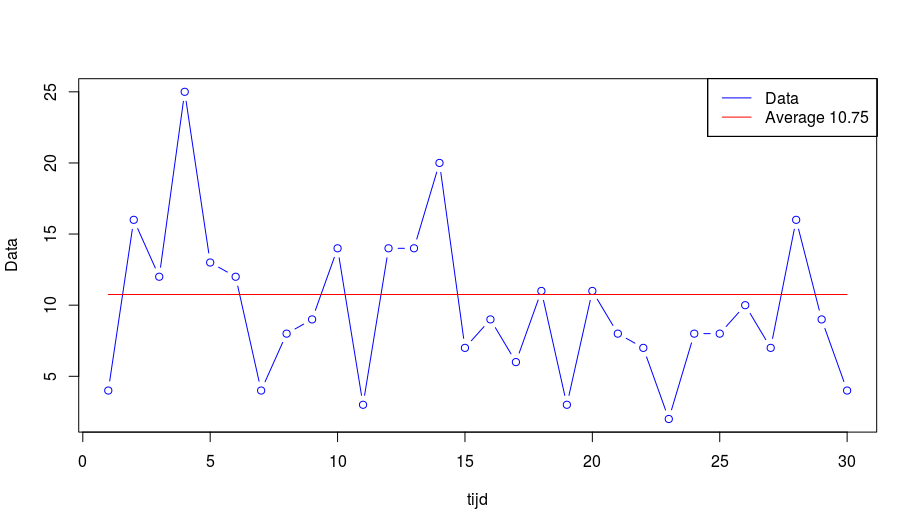
\includegraphics[width=1.00\textwidth]{images/tijdreeksen/tijdreeks20.png}
	\caption{Tijdreeks met constant gemiddelde $10.75$}
	\label{fig:tijdreeks21}
\end{figure}

Indien we veronderstellen dat de data verandert met de tijd is het beter om oude data minder te laten meetellen dan recentere. Een mogelijkheid is om enkel recente data te gebruiken, bijvoorbeeld de 10 of 5 laatste datapunten (zie figuur \ref{fig:tijdreeks31}).

\[ \widehat{b} = \frac{1}{10} \sum_{10}^{20} x_{t} = 10.18 \] en
\[ \widehat{b} = \frac{1}{5} \sum_{15}^{20} x_{t} = 7.83 \]

\begin{lstlisting}
sma10 <- SMA(x =data,n=10)
sma5 <- SMA(x=data,n=5)
plot.ts(x = data, col = 'blue',type = 'l')
lines(sma10, col='red', type = 'b')
lines(sma5, col='purple', type = 'b')
\end{lstlisting}

\begin{figure}
\centering
	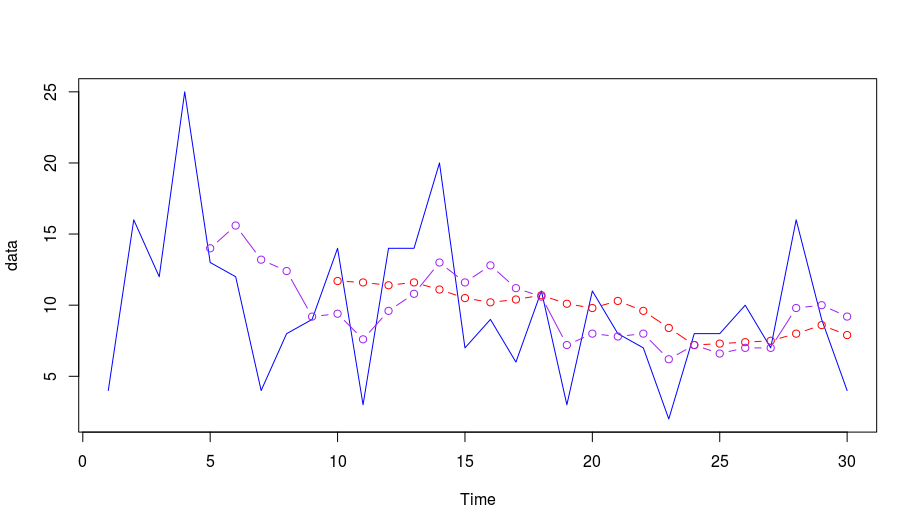
\includegraphics[width=1.00\textwidth]{images/tijdreeksen/tijdreekssma.png}
	\caption{Tijdreeks met voortschrijdend gemiddelde $m = 10$ en $m=5$}. 
\label{fig:tijdreeks31}
\end{figure}

Dit worden \textit{voortschrijdende gemiddelden}\index{voortschrijdend gemiddelde} genoemd (Eng. \emph{moving average}). 

Welke schatter is nu de beste? We kunnen dit nu nog niet zeggen.

\begin{itemize}
\item De schatter die alle datapunten gebruikt is de beste indien de tijdreeks het model volledig volgt.
\item De schatter met de recentere datapunten is de beste indien de tijdreeks verandert met de tijd.
\end{itemize}

\begin{definition}[voortschrijdend gemiddelde]
Algemeen is het \emph{voortschrijdend gemiddelde} (Eng. \emph{moving average}) het gemiddelde van de $m$ laatste observaties.
\begin{equation}
	\widehat{b} = \sum_{i=k}^{t} \frac{x_{i}}{m}
\label{eq:movingAverage}
\end{equation}
met $k = t-m+1$. $m$ is de time range en is de parameter van de methode.
\end{definition}

\subsection{Meten van de nauwkeurigheid van voorspellingen}

\begin{table}
  \centering
\begin{tabular}{|lllllllllll|}

\end{tabular}
\caption{Voorspellingsfout voor een moving average $m = 10$}
\label{tab:error}
\end{table}


Een methode om de voorspelling te meten is het gemiddelde van de deviaties (Eng.~\emph{Mean Average Deviation}, afgekort $MAD$): gemiddelde absolute verschil tussen het voorspelde en de werkelijke waarden van de tijdreeks.

\begin{definition}[$MAD$]
\begin{equation}
	MAD = \frac{1}{n} \sum_{1}^{n} \left| e_{i} \right|  
\label{eq:MAD}
\end{equation}
\end{definition}

Je kan dit ook percenteren om zo tot de gemiddelde absolute procentuele afwijking (Eng.~\emph{Mean Absolute Percentage Error}, afgekort $MAPE$) te komen.

\begin{definition}[$MAPE$]
\begin{equation}
	MAPE = \frac{1}{n} \sum_{1}^{n} \left| \frac{e_{i}}{X_i} \right|  
\label{eq:MAD2}
\end{equation}
\end{definition}

Je kan ook de variantie van de fouten bepalen:

\begin{definition}[$VAR$]
\begin{equation}
	s^{2}_{e} = \frac{1}{m} \sum_{1}^{n} (e_{i} - \overline{e})^{2}
\label{eq:varError}
\end{equation}
\end{definition}

% TODO: moet de noemer hierboven niet n - 1 zijn??

Als laatste interessante parameter kan gekeken worden naar de wortel uit de gemiddelde kwadratische afwijking (Eng.~\emph{root-mean-squared error}, afgekort $RMSE$), als de wortel uit het gemiddelde gekwadrateerde verschil tussen de voorspelde en de werkelijke waarden van de tijdreeks.

\begin{definition}[$RMSE$]
\begin{equation}
	RMSE_{e} = \sqrt{\frac{1}{m} \sum_{1}^{n} (e_{i})^{2}}
\label{eq:varError2}
\end{equation}
\end{definition}

\section{Exponentiële afvlakking}

Bij een voortschrijdend gemiddelde krijgen alle voorgaande observaties een gelijk gewicht. Bij exponentiële afvlakking (Eng. \emph{exponential smoothing}) worden kleinere gewichten toegekend aan oudere observaties. Met andere woorden, recentere observaties krijgen relatief meer gewicht dan oudere observaties.

In het geval van het eenvoudig voortschrijdend gemiddelde zijn de gewichten hetzelfde, namelijk $\frac{1}{m}$.

\subsection{Enkelvoudige exponentiële afvlakking}

Exponentiële afvlakking is een gewogen gemiddelde dat positieve gewichten toekent aan de huidige waarden en waarden uit het verleden van de tijdreeks. Een enkel gewicht, $0\leq \alpha \leq1$ of de afvlakkingsconstante (Eng.~\emph{smoothing constant}) wordt hiervoor gekozen. Voor een tijdseenheid $t$ wordt de enkelvoudige exponentiële afvlakking gevonden door vergelijking \ref{eq:singleExpSmooting}.

\begin{definition}[Exponentiële afvlakking]
\begin{equation}
	X_{t} = \alpha x_{t} + (1-\alpha)X_{t-1}, 0 \leq \alpha \leq 1, t \geq 3
\label{eq:singleExpSmooting}
\end{equation}
\end{definition}

Met andere woorden, $X_{t}$ is een gewogen gemiddelde van de huidige waarneming $x_t$ en de vorige exponentiële afvlakking $X_{t-1}$.

\subsubsection{Intiële setting}
Het bepalen van $X_{2}$ is een belangrijke parameter. Men kan kiezen om:
\begin{enumerate}
	\item $X_{2} = x_{1}$ te stellen
	\item $X_{2}$ gelijk te stellen aan een bepaald objectief
	\item Een gemiddelde te nemen van de eerste $x$ observaties
	\item \dots
\end{enumerate}

Waarom wordt dit een exponentiële methode genoemd? Als we zouden substitueren vinden we bv. voor $X_{t-1}$:

\[ X_{t} = \alpha x_{t} + (1-\alpha)\left[\alpha x_{t-1} + (1-\alpha)X_{t-2}\right] \] 
\[ X_{t} = \alpha x_{t-1} + \alpha (1-\alpha)x_{t-1} + (1-\alpha)^{2} X_{t-2} \]
of dus algemeen gesteld :
\[ X_{t} = \alpha \sum_{i=0}^{t-2}(1-\alpha)^{i-1}x_{t-i} + (1-\alpha)^{t-2} X_{2}, t \geq 2 \]

Zo merk je dat oudere componenten een exponentieel kleiner gewicht verkrijgen. 

\subsubsection{Waarde voor $\alpha$}
De snelheid waarmee de oude observaties ''vergeten`` worden hang af van $\alpha$. Met een $\alpha$ dicht bij 1 vergeet je snel, terwijl een $\alpha$ dicht bij nul ervoor zorgt dat vergeten minder snel gaat (zoals aangetoond in tabel \ref{tab:alpha}). Vaak wordt een waarde gebruikt tussen $0.10$ en $0.30$.

\begin{table}
\centering
    \begin{tabular}{l|llll}
    $\alpha$ & $(1-\alpha)$ & $(1-\alpha)^{2}$ & $(1-\alpha)^{3}$ & $(1-\alpha)^{4}$ \\ \hline
    0.9   & 0.1       & 0.01             & 0.001                      & 0.0001           \\
    0.5   & 0.5       & 0.25             & 0.125                      & 0.062            \\
    0.1   & 0.9       & 0.81             & 0.729                      & 0.6561           \\
    \end{tabular}
		\caption{Waarden voor $\alpha$ en $(1-\alpha)^{n}$}
		\label{tab:alpha}
\end{table}

Bijvoorbeeld, het bestand \texttt{precip.data} bevat totale jaarlijkse neerslag in inches voor Londen, vanaf 1813-1912. Laten we dit eens analyseren met R.

\begin{lstlisting}
rain <- scan("cursus/data/tijdreeksen/precip.data",skip=1)
rainseries <- ts(rain,start=c(1813))
plot.ts(rainseries)
plot(rainseriesforecasts)
\end{lstlisting} 

%TODO figuur maken voor verschillende alpha's

\subsubsection{Voorspelling met exponentiële effening}

Stel dat het doel is om de volgende waarde $X_{t+1}$ te voorspellen, dan wordt dit gelijk gesteld aan de afvlakkingswaarde op tijdstip $t$.

\begin{equation}
	X_{t+1} = EMA_t = X_t
	\label{eq:EMA}
\end{equation}

Met $X_t$ de laatst voorspelde waarde. 

We kunnen dit eenvoudig uitvoeren in R. Je krijgt hierbij een \emph{prediction interval}, een interval waarin we verwachten dat de voorspelde waarde met een bepaalde waarschijnlijkheid zal liggen. Standaard krijg je een 80\% en een 95\% interval.

\begin{lstlisting} 
library('forecast')
rainseriesforecasts2 <- forecast.HoltWinters(rainseriesforecasts, h=8)
plot.forecast(rainseriesforecasts2)
\end{lstlisting} 

We zouden correlaties mogen zien tussen de voorspellingsfouten voor opeenvolgende voorspellingen. Met andere woorden, als er sprake is van een correlatie tussen prognosefouten voor opeenvolgende voorspellingen, is het eerder waarschijnlijk dat de simpele exponentiële afvlakking kan worden verbeterd door een andere voorspellingstechniek te gebruiken.

Om te achterhalen of dit het geval is, kunnen we een correlogram verkrijgen van de in-sample voorspellingsfouten voor.

We weten nog uit hoofdstuk~\ref{ch:analyse2var} dat de covariantie of correlatie de lineaire relatie beschrijft tussen twee variabelen. De autocovariantie en autocorrelatie meten de lineaire relatie tussen in de tijd verschoven waarden voor een tijdreeks.

\begin{definition}[Autocovariantie]
	We definiëren de autocovariantie bij vertraging $k$ door $c_k$.
	\[ c_k = \sum_{t=k+1}^{T} (y_t - \overline{y})(y_{t-k} - \overline{y}) \]
\end{definition}

\begin{definition}[Autocorrelatie]
	We definiëren de autocorrelatie bij vertraging $k$ door $r_k$.
	\[ r_k = \frac{c_k}{c_0} \]
\end{definition}

Een correlogram is een grafiek van de autocorrelaties. In R kan je die plotten met de functie \texttt{acf()}. Deze berekent ook de voorspellingsfouten. Om de maximale vertraging te bepalen die we willen bekijken, gebruiken we de parameter \texttt{lag.max}.

Bijvoorbeeld, om een correlogram te berekenen van de prognosefouten voor de Londen-regenvalgegevens voor vertragingen 1 tot en met 20, typen we:

\begin{lstlisting}
acf(rainseriesforecasts2$residuals, lag.max=20, na.action = na.pass)
\end{lstlisting}

Om te testen of er significant bewijs is voor significante correlaties bij vertraging 1-20, kunnen we een Ljung-Box test uitvoeren. Dit kan in R worden gedaan met de functie \texttt{Box.test()}. De maximale vertraging die we willen bekijken, wordt gespecificeerd met behulp van de parameter \texttt{Lag}.

De test volledig uitleggen valt buiten het bereik van deze cursus, maar de test gaat uit van de hieronder geformuleerde hypothesen $H_0$ en $H_1$. De teststatistieken kunnen dan gewoon geïntepreteerd worden zoals alle andere hypothesetesten die beschreven geweest zijn in vorige hoofdstukken. 

\begin{itemize}
  \item $H_0$ De gegevens zijn onafhankelijk verdeeld (d.w.z. de correlaties in de populatie waaruit de sample wordt genomen, zijn 0, zodat elke waargenomen correlatie in de data voortvloeien uit willekeurigheid).
  \item $H_1$ De gegevens zijn niet onafhankelijk verdeeld: ze tonen een linaire correlatie.
\end{itemize}

Bijvoorbeeld, om te testen of er geen nul autocorrelaties zijn op vertragingen 1-20, voor de in-sample voorspellingen fouten voor Londen regenval data, typen we:

% TODO: correcte Nl term voor in-sample error?

\begin{lstlisting}
Box.test(rainseriesforecasts2$residuals, lag=20, type="Ljung-Box")
Box-Ljung test
data:  rainseriesforecasts2$residuals
X-squared = 17.4008, df = 20, p-value = 0.6268
\end{lstlisting}

Als laatste moeten we ook kijken naar de verdeling van de fouten van de voorspelling. Zoals boven vermeld gaan we ervan uit dat de fouten normaal verdeeld zijn met een gemiddelde $\mu = 0$ en een standaardafwijking die constant is. Om deze veronderstelling te controleren, kunnen we een histogram van de prognosefouten plotten, met een overlappende normale curve met gemiddelde nul en dezelfde standaardafwijking heeft als de verdeling van de voorspellingsfouten. Hiervoor kunnen we een R-functie \texttt{plotForecastErrors()} definiëren. Het is ook aangewezen de methoden zoals beschreven in sectie~\ref{sec:normtesting}.

% TODO: zin onvolledig

\begin{lstlisting}
plotForecastErrors <- function(forecasterrors)
{
# make a histogram of the forecast errors:
mybinsize <- IQR(forecasterrors)/4
mysd   <- sd(forecasterrors)
mymin  <- min(forecasterrors) - mysd*5
mymax  <- max(forecasterrors) + mysd*3
# generate normally distributed data with mean 0 and standard deviation mysd
mynorm <- rnorm(10000, mean=0, sd=mysd)
mymin2 <- min(mynorm)
mymax2 <- max(mynorm)
if (mymin2 < mymin) { mymin <- mymin2 }
if (mymax2 > mymax) { mymax <- mymax2 }
# make a red histogram of the forecast errors, with the normally distributed data overlaid:
mybins <- seq(mymin, mymax, mybinsize)
hist(forecasterrors, col="red", freq=FALSE, breaks=mybins)
# freq=FALSE ensures the area under the histogram = 1
# generate normally distributed data with mean 0 and standard deviation mysd
myhist <- hist(mynorm, plot=FALSE, breaks=mybins)
# plot the normal curve as a blue line on top of the histogram of forecast errors:
points(myhist$mids, myhist$density, type="l", col="blue", lwd=2)
}
\end{lstlisting}

\subsection{Dubbele exponentiële afvlakking}

Enkelvoudige afvlakking wordt gebruikt wanneer er geen trend zichtbaar is. Wanneer er een trend (stijgend of dalend) is dan kan er iets fout gaan. Zie bijvoorbeeld de data in tabel~\ref{tab:trend} en figuur~\ref{fig:tijdreeks61}.

\begin{table}
\centering
    \begin{tabular}{|ll|}
    \hline
    Data & Enkelvoudige afvlakking \\
    6.4  & ~                      \\
    5.6  & 6.4                    \\
    7.8  & 6.2                    \\
    8.8  & 6.7                    \\
    11.0 & 7.3                    \\
    11.6 & 8.4                    \\
    16.7 & 9.4                    \\
    15.3 & 11.6                   \\
    21.6 & 12.7                   \\
    22.4 & 15.4                   \\ \hline
    \end{tabular}
		\caption{Enkelvoudige afvlakking met $\alpha = 0.3$}
		\label{tab:trend}
\end{table}

\begin{figure}
  \centering
  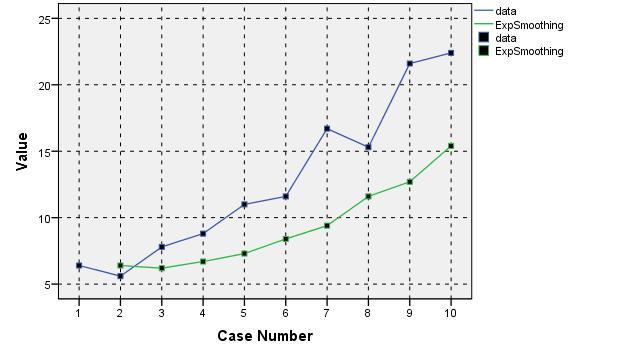
\includegraphics[width=1.00\textwidth]{images/tijdreeksen/tijdreeks61.jpg}
  \caption{Exponentiële afvlakking bij een trend}
  \label{fig:tijdreeks61}
\end{figure}

Daarom voegen we een extra constante toe om deze trap te overbruggen:

\begin{definition}[Holt-voorspelling of dubbele exponentiële afvlakking]
\begin{eqnarray}
	X_{t} = \alpha x_{t} + (1-\alpha)(X_{t-1} + b_{t-1}) & 0 \leq \alpha \leq 1 \\
	b_{t} = \gamma(X_{t}-X_{t-1}) + (1-\gamma)b_{t-1} & 0 \leq \gamma \leq 1 
\label{eq:doubleSmoothing}
\end{eqnarray}
\end{definition}

\subsubsection{Initiële waarde}

Net zoals in enkelvoudige afvlakking kan je verschillende methodes kiezen om initiële waardes voor $X_{t}$ en $b_{t}$ te kiezen:

\begin{itemize}
	\item $X_{1} = x_{1}$
	\item $b_{1} = x_{2} - x_{1}$
	\item $b_{1} = \frac{1}{3}\left[ (x_{2} - x_{1}) + (x_{1} - x_{2}) + (x_{4} - x_{3}) \right]$
	\item $b_{1} = \frac{x_{n} - x_{1}}{n-1}$
\end{itemize}

\subsubsection{Voorspelling}

Een voorspelling maken met dubbele exponentiële afvlakking gebeurt dan iets anders (noem $F_{t+1}$ de voorspelling voor tijd $T+1$):

\[ F_{t+1} = X_{t} + b_{t} \]
of
\[ F_{t+m} = X_{t} + m b_{t} \]

Als we nu de tekening maken met enkelvoudige afvlakking ($\alpha = 0.977$) en dubbele afvlakking ($\alpha = 0.3623, \gamma = 1.0, X_{1} = x_{1} = 6.4$ en $b_{1} = \frac{1}{3}\left[ (x_{2} - x_{1}) + (x_{1} - x_{2}) + (x_{4} - x_{3}) \right] = 0.8$ vinden we volgende waarden in tabel \ref{tab:doubleSingle} en figuur \ref{fig:tijdreeks71}:

\begin{table}
  \centering
  \begin{tabular}{|llll|}
    \hline
    Data & Enkelvoudige afvlakking $X_{t}$ & Double afvlakking $X_{t}$ & $F_{t}$ \\
    6.4  & ~                      & 6.4              & ~                             \\
    5.6  & 6.4                    & 6.6              & 7.2                           \\
    7.8  & 5.6                    & 7.2              & 6.8                           \\
    8.8  & 6.7                    & 8.1              & 7.8                           \\
    11.0 & 8.8                    & 9.8              & 9.1                           \\
    11.6 & 10.9                   & 11.5             & 11.4                          \\
    16.7 & 11.6                   & 14.5             & 13.2                          \\
    15.3 & 16.6                   & 16.7             & 17.4                          \\
    21.6 & 15.3                   & 19.9             & 18.9                          \\
    22.4 & 21.5                   & 22.8             & 23.1                          \\ \hline
  \end{tabular}
  \caption{Tabel met enkelvoudige en dubbele afvlakking}
  \label{tab:doubleSingle}
\end{table}

\begin{figure}
	\centering
		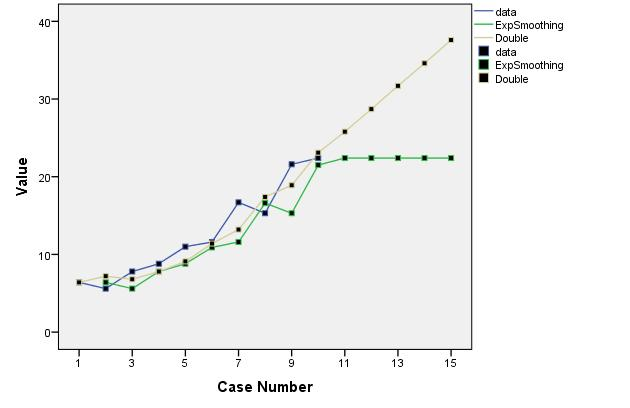
\includegraphics[width=1.00\textwidth]{images/tijdreeksen/tijdreeks71.jpg}
	\caption{Enkelvoudige en dubbele afvlakking}
	\label{fig:tijdreeks71}
\end{figure}

De manier om dit met R op te lossen is gelijkaardig als bij exponentiële afvlakking, alleen moet de parameter gamma $\gamma$ niet op NULL gezet worden. Het maken van de correlogram, de Ljung–Box test en het testen van de normaliteit van de errors gebeurt om dezelfde manier. 

\subsection{Driedubbele exponentiële afvlakking}

In vele tijdreeksen zie je bepaalde patronen terugkomen. Neem bijvoorbeeld is de dagelijkse omzet van een bakker: die zal elke dag anders zijn, maar als je die over een lange periode bekijkt, zal je wellicht elke week een gelijkaardig patroon terugzien (met bv. een topomzet op zondag).

Dit soort tijdreeksen kan benaderd worden met de Holt-Winters methode, of driedubbele exponentiële afvlakking.

\begin{eqnarray}
  X_{t} = \alpha \frac{x_{t}}{c_{t-L}} + (1-\alpha) (X_{t-1} + b_{t-1}) & \textnormal{Smoothing}\\
  b_{t} = \gamma (X_{t} - X_{t-1}) + (1-\gamma)b_{t-1} & \textnormal{Trend smoothing} \\
  c_{t} = \beta \frac{x_{t}}{X_{t}} + (1-\beta)c_{t-L} & \textnormal{Seasonal smoothing} \\
  F_{t+m} = (X_{t} + mb_{t})c_{t-L+m \mod L}  & \textnormal{Voorspelling}
  \label{eq:HoltWinters}
\end{eqnarray}
 met 
\begin{itemize}
	\item $x_{t}$ de observatie op tijdstip $t$
	\item $X_{t}$ is de afgevlakte observatie op tijdstip $t$
	\item $b_{t}$ is de trendfactor op tijdstip $t$
	\item $c_{t}$ is de seizoensindex op tijdstip $t$
	\item $F_{t}$ is de voorspelling op tijdstip $t$
	\item $L$ is de periode (bv. van de seizoenen)
\end{itemize}

$\alpha, \beta en \gamma$ zijn constanten die geschat moeten worden. 
De manier om dit met R op te lossen is gelijkaardig als bij exponentiële afvlakking. Het maken van de correlogram, de Ljung–Box test en het testen van de normaliteit van de errors gebeurt op dezelfde manier. 

\section{Oefeningen}
\label{sec:tijdreeksen-oefeningen}

\begin{exercise}
In bijgevoegd bestand \emph{Budget.csv} vind je vanaf 1981 tot 2005 per kwartaal de omzet, het advertentiebudget en het BNP van een middelgroot bedrijf. Voeg zelf nog een kolom 'Kwartaalnummer' toe.

\begin{enumerate}
  \item Bereken het voortschrijdend gemiddelde \emph{(simple moving average)} over de periodes 4 en 12 voor deze data. Gebruik hiervoor de methode SMA. Maak een lijngrafiek van $X$, $SMA(4)$ en $SMA(12)$.
  \item Welke techniek die we eerder gezien hebben (in het deel over beschrijvende statistiek) is ook geschikt om voorspellingen te maken over de waarden van $X$? Werk dit uit aan de hand van de daarvoor bestemde functie en plot het resultaat in de grafiek.
  \item Gebruik de methode \emph{forecast} om voorspellingen voor de 10 volgende periodes met elk van voorgaande methoden (dus moving average 4 en 10 en regressie) te maken. Teken deze eveneens op de grafiek.
  \item Is het gebruik van één van deze technieken interessant om voor deze data voorspellingen te maken? 
  \item Maak van de data een tijdreeks via de methode \emph{ts}. Gebruik de methode \emph{decompose} om de tijdreeks op te delen en zo een idee te krijgen van de trend en de seizoenschommeling.
  \item Bereken het exponentieel voortschrijdend gemiddelde \emph{(exponential moving average, EMA)} door gebruik te maken van de methode \emph{HoltWinters}. Maak opnieuw via de methode \emph{forecast} een voorspelling voor 20 periodes. Gebruik als startwaarden $s_1 = x_1$ en $\alpha $ de door R gegenereerde waarde. Plot het resultaat op een nieuwe grafiek samen met $X$.
  \item Doe nu hetzelfde met $\alpha=0.1$. 
  \item Hoe zien de voorspellingen er nu uit?
  \item Doe nu hetzelfde met \emph{dubbele} exponentiële afvlakking. Gebruik als startwaarden $s_1 = x_1$ en $b_1 = \frac{x_n - x_1}{n - 1}$, $\alpha =  0.05$ en $\beta = 0.2$. Plot het resultaat op de grafiek.
  \item Gebruik dubbele exponentiële afvlakking om voorspellingen te berekenen voor 20 periodes. Plot de waarden op de grafiek. Is deze techniek beter of slechter dan de vorige voor deze dataset?
  \item Speel met de waarden voor $\alpha$ en $\beta$ en bekijk het resultaat, zowel voor enkele als dubbele exponentiële afvlakking.
  \item Gebruik de \emph{HoltWinters}-methode zonder trend.  M.a.w. we stellen $\beta=0$. Gebruik als startwaarden $\alpha =  0.05$ en $\gamma = 0.9$. Plot het resultaat op de grafiek.
  \item Bereken opnieuw voorspellingen voor 20 periodes. Plot de waarden op de grafiek. Is deze techniek beter of slechter dan de vorige voor deze dataset?
  \item Speel met de waarden voor $\alpha$, $\beta$ en $\gamma$ en bekijk het resultaat.
  \item Gebruik de \emph{HoltWinters}-methode met de door R-gegeneerde waarden zonder trend.  M.a.w. we stellen $\beta=0$.  Plot het resultaat op de grafiek.
  \item Bereken opnieuw voorspellingen voor 20 periodes maar gebruik nu de methode \emph{predict}. Plot de waarden op de grafiek. Is deze techniek beter of slechter dan de vorige voor deze dataset?
\end{enumerate}	
\end{exercise}

\begin{exercise}
In bestand \emph{Passagiers2.csv} vind je vanaf januari 1949 tot december 1960 het aantal passagiers van een luchtvaartmaatschappij. 
\begin{enumerate}
  \item Bereken het voortschrijdend gemiddelde \emph{(simple moving average)} over de periodes 4 en 12 voor deze data. Gebruik hiervoor de methode \emph{ma}. Maak een lijngrafiek van $X$, $MA(4)$ en $MA(12)$.
  \item Welke techniek die we eerder gezien hebben (in het deel over beschrijvende statistiek) is ook geschikt om voorspellingen te maken over de waarden van $X$? Werk dit uit aan de hand van de daarvoor bestemde functie en plot het resultaat in de grafiek.
  \item Gebruik de methode \emph{forecast} om voorspellingen voor de 10 volgende periodes met elk van voorgaande methoden (dus moving average 4 en 10 en regressie) te maken. Teken deze eveneens op de grafiek. Conclusie?
  \item Is het gebruik van één van deze technieken interessant om voor deze data voorspellingen te maken? 
  \item Gebruik de methode \emph{decompose} om de tijdreeks op te delen en zo een idee te krijgen van de trend en de seizoenschommeling.
  \item Bereken het exponentieel voortschrijdend gemiddelde \emph{(exponential moving average, EMA)} door gebruik te maken van de methode \emph{ses} met $\alpha=0.2$. Maak opnieuw via de methode \emph{forecast} een voorspelling voor 20 periodes. Plot het resultaat op een nieuwe grafiek samen met $X$.
  \item Doe nu hetzelfde met $\alpha=0.6$ en $\alpha=0.89$. 
  \item Hoe zien de voorspellingen er nu uit?
  \item Doe nu hetzelfde met \emph{dubbele} exponentiële afvlakking. Gebruik hiervoor de methode \emph{holt}  $\alpha =  0.8$ en $\beta = 0.2$. Plot het resultaat op de grafiek.
  \item Gebruik dubbele exponentiële afvlakking om voorspellingen te berekenen voor 20 periodes. Plot de waarden op de grafiek. Is deze techniek beter of slechter dan de vorige voor deze dataset?
  \item Gebruik in de methode de optie $exponential=TRUE$. Teken het resultaat.  Wat is het verschil?
  \item Gebruik de \emph{hw}-methode met de door R gegeneerde waarden. Plot het resultaat op de grafiek.
  \item Bereken opnieuw een aantal voorspellingen via de methode \emph{predict}. Plot de waarden op de grafiek. Is deze techniek beter of slechter dan de vorige voor deze dataset?
  \item Speel met de waarden voor $\alpha$, $\beta$ en $\gamma$ en bekijk het resultaat.
\end{enumerate}

\end{exercise}